\documentclass{beamer}
\usepackage[english]{babel}
%\usepackage[utf8x]{inputenc}
\usepackage{ctex,
			hyperref, % clickable links
   			graphicx, % include images
		    listings, % for code and formatting
		    caption, % customization of captions in figures and tables
		    subcaption,%自定义子标题
		    stackengine, % custom layouts 
		    amsmath, % math env
		    xcolor, % extend color support
		    multicol, % multiple columns layout
		    booktabs, % high quality tables
		    lipsum , % remove it
		    calligra,%最后字体thank you!
		    url,%链接
		   setspace,
		   }
%\beamerdefaultoverlayspecification{<+->}
\setbeamercovered{transparent}%透明transparent=20 20%透明度
\usepackage{CHD_beamer} % customized style
\usefonttheme[onlymath]{serif}%设置斜体


\def\cmd#1{\texttt{\color{red}\footnotesize $\backslash$#1}}
\def\env#1{\texttt{\color{blue}\footnotesize #1}}

% ------ CODE COLOR DEFINITION ------ %

\definecolor{codered}{rgb}{0.6,0,0}
\definecolor{codeblue}{rgb}{0,0,0.8}
\definecolor{codegreen}{rgb}{0,0.5,0}
\definecolor{almostwhite}{gray}{0.55}
\definecolor{codepurple}{rgb}{271,36,28}
\definecolor{backcolour}{rgb}{0.95,0.95,0.92}

% ------------- PRESENTATION INFO --------------- %
\newcommand{\fullconference}{}%指导老师:李辉
\newcommand{\shortconference}{汇报}
\newcommand{\contact}{\textit{}}%luwenke@chd.edu.cn

\author[\text{路文科}~luwenke420@outlook.com\contact]{\href{}{路文科}}%在\text{路文科} \contact中加入邮箱参考newcommand中\textit{luwenke@chd.edu.cn}
\institute[\text{材料科学与工程学院}]{\href{}{Chang'an University}
    \\ \smallskip \contact}
\title[]%Short titl“路文科”下边的标题
{这学期我做了什么}
\subtitle[\shortconference]{}%子标题
\date[\today]{\fullconference
    \\ \small \today}


\begin{document}

% ------------ TITLE SLIDE --------------- %
{
% Remove headline and footline from first slide
\setbeamertemplate{footline}{} 
\setbeamertemplate{headline}{} 

\begin{frame}\label{start}
    \titlepage
    \begin{figure}
            
\includegraphics[scale=0.03]{style/chdbluelogo.pdf} 
    \end{figure}
\end{frame}
}

% ---------- TABLE OF CONTENT --------- %
\begin{frame}{目录}
    \tableofcontents[sectionstyle=show, subsectionstyle=show/shaded/hide, subsubsectionstyle=show/shaded/hide]
\end{frame}


\section{python画图}

\begin{frame}{python画图}
	
    \begin{block}{python画图}
    	形成模板以后画DOS图时只需要简单的运行程序就能够得到一张DOS矢量图\\
    	其他的图暂时没有接触到以后有待补充
    \end{block}
      例:
      
	\begin{figure}
		\centering
		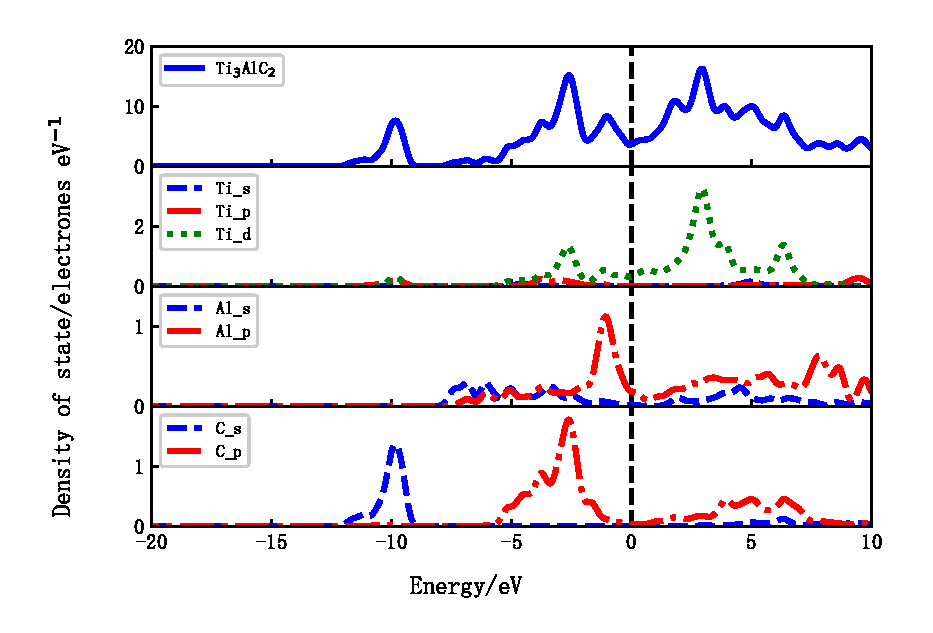
\includegraphics[width=5cm]{images/Figure_1.eps}
		\caption{$Ti_{3}AlC_{2}-GGA~PBE$}
		\label{fig:Figure_1}
	\end{figure}
\end{frame}



\section{学习\LaTeX{}}

	\begin{frame}{\LaTeX{} ?}
		\begin{block}{\LaTeX{}是什么?}
			\begin{itemize}[<+->]
				\item 它是一种高质量的排版工具,能够通过代码来自动控制排版,对于长篇幅的文章来说非常适合。并且能够形成模板化的工具。
				\item 最擅长数学公式排版
				\item 优点:开源,免费 
				\item 资源中心:\url{www.ctan.org}
				\item 论坛:\url{www.latexstudio.net}
			\end{itemize}
			
		\end{block}
		\pause
		\begin{exampleblock}{我用它做了什么?}
			\begin{description}
				\item[1] 写科技论文
				\item[2] 做演示模板
				\item[3] 写毕业论文
			\end{description}
		\end{exampleblock}		
	\end{frame}	
	
	\begin{frame}{\LaTeX 示例}
			\begin{table}[]
				\caption{这是一个表格}
				\resizebox{\textwidth}{!}{
					\begin{tabular}{|c|c|c|c|c|c|c|c|c|c|c|c|c|c|c|}
							\hline
							MAX     & Method  & $C_{11}$   & $C_{33}$   & $C_{44}$   & $C_{12}$  & $C_{13}$   & $B_{V}$    & $B_{R}$    & $B_{H}$    & $G_{V}$    & $G_{R}$    & $G_{H}$    & $E$     & $v$     \\ \hline
							$Ti_{3}SiC_{2}$ & LDA     & 409.9 & 389.9 & 175.5 & 95.3 & 112.2 & 205.4 & 205.4 & 205.4 & 161.0 & 159.8 & 160.4 & 381.8 & 0.190 \\ \hline
							& GGA-PBE & 336.5 & 343.7 & 153.8 & 97.1 & 99.4  & 178.8 & 178.7 & 178.7 & 133.5 & 131.5 & 132.5 & 387.7 & 0.203 \\ \hline
							$Ti_{3}AlC_{2}$ & LDA     & 388.3 & 320.3 & 138.4 & 83.8 & 77.4  & 174.9 & 173.4 & 174.1 & 143.0 & 142.4 & 142.7 & 336.2 & 0.178 \\ \hline
							& GGA-PBE & 354.6 & 288.7 & 121.4 & 72.5 & 67.6  & 157.0 & 155.5 & 156.3 & 129.4 & 128.5 & 129.0 & 303.4 & 0.176 \\ \hline
						\end{tabular}
										}		
			\end{table}
			
\begin{columns}
	
\column{0.4\textwidth}
	\begin{itemize}
		\item 这是dos
		\item 这是dos 
		\begin{itemize}
			\item 这也是dos
		\end{itemize}
	\end{itemize}	
				
\column{0.6\textwidth}
	\begin{columns}
		
	\column{0.5\textwidth}
		\begin{figure}
			\centering
			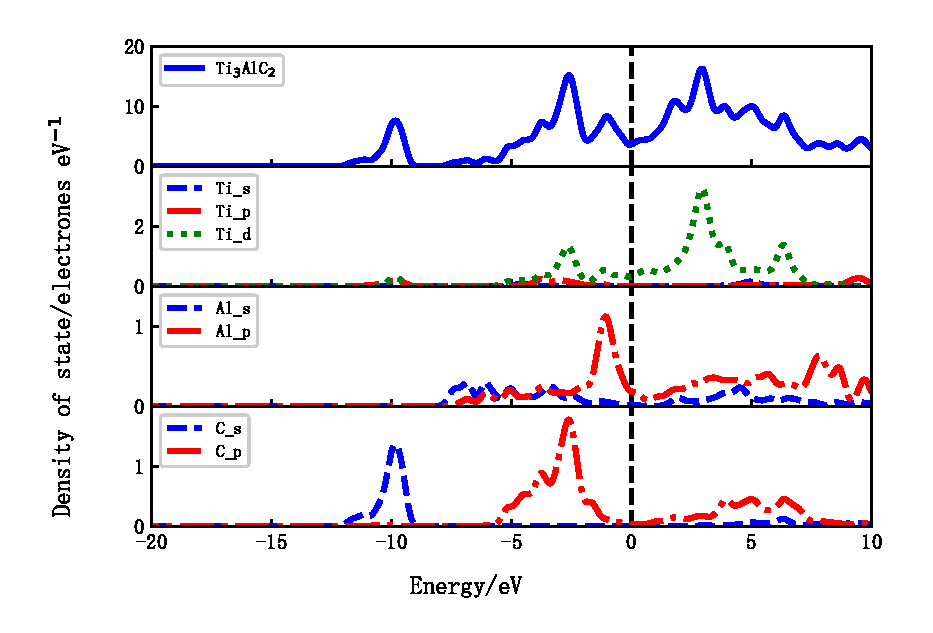
\includegraphics[width=3.5cm]{images/Figure_1.eps}
			%\caption{}
			\label{fig:Figure1}
		\end{figure}
	
	\column{0.5\textwidth}
	\hspace{0.1cm} 
		\begin{figure}
			\centering
			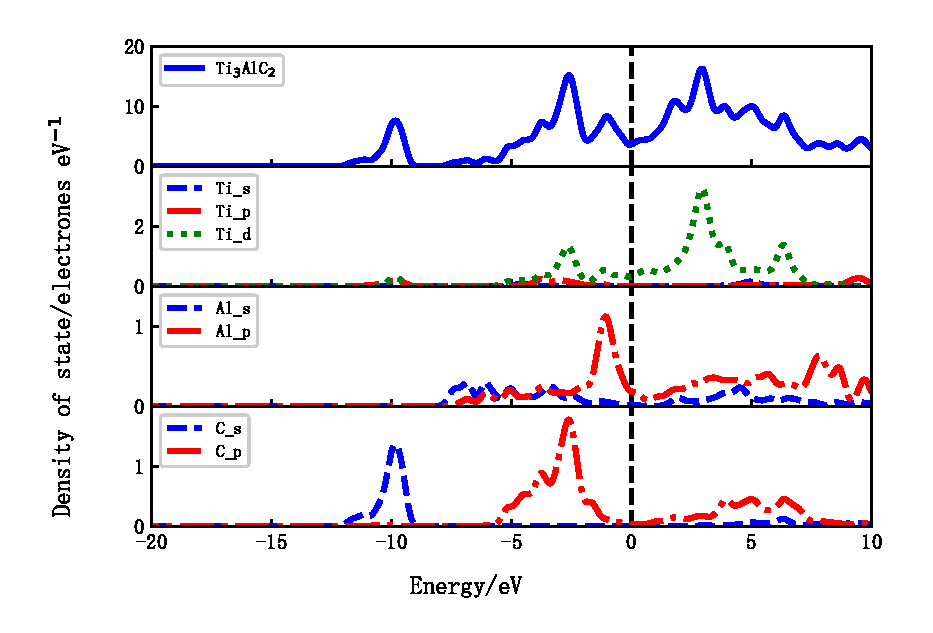
\includegraphics[width=3.5cm]{images/Figure_1.eps}
			%\caption{}
			\label{fig:Figure2}
		\end{figure}
	\end{columns}
				
\end{columns}
	\end{frame}

\begin{frame}{数学公式}
	\begin{columns}
		\begin{column}{0.5\textwidth}
			\begin{equation}
				x = \frac{-b \pm \sqrt{\Delta}}{2a}
				\label{eq:equation1}
			\end{equation}
	
				\begin{align}
					x &= y + z \\
					a &= b - c
				\end{align}

		\end{column}
	
		\begin{column}{0.5\textwidth}
			\begin{equation}
				\left\lbrace 
				\begin{aligned}
					\mathit{x} &= \mathit{y + z} \\
					\mathit{a} &= \mathit{b - c}
				\end{aligned}
				\right. 
			\end{equation}
			\begin{gather}
					\mathit{x = y + z} \\
					\mathit{a = b - c} \nonumber \\
					\mathit{E = mc^2}
			\end{gather} 
		\end{column}		
	\end{columns}
				
		 在公式~\ref{eq:equation1}中,~\dots 众所周知$sin^2x+cos^2x = 1$这是一个三角函数。$e^{i\varphi}=\cos \varphi +i\sin \varphi $,$e^{i\pi}+1=0$公式和文字之间毫无违和感$\hat{f}\left( \xi \right) =\int_{-\infty}^{\infty}{f\left( x \right) e^{-2\pi ix\xi}\text{d}x}$\footnote[frame]{傅里叶变换}积分\dots,$i\hbar \frac{\partial}{\partial t}\Psi(r,t) = \hat{H}\Psi(r,t)$\footnote[frame]{薛定谔方程}。对上述文字word排版差点意思。
			
\end{frame}	

\begin{frame}{例}
		\begin{figure}[h]
			\centering
			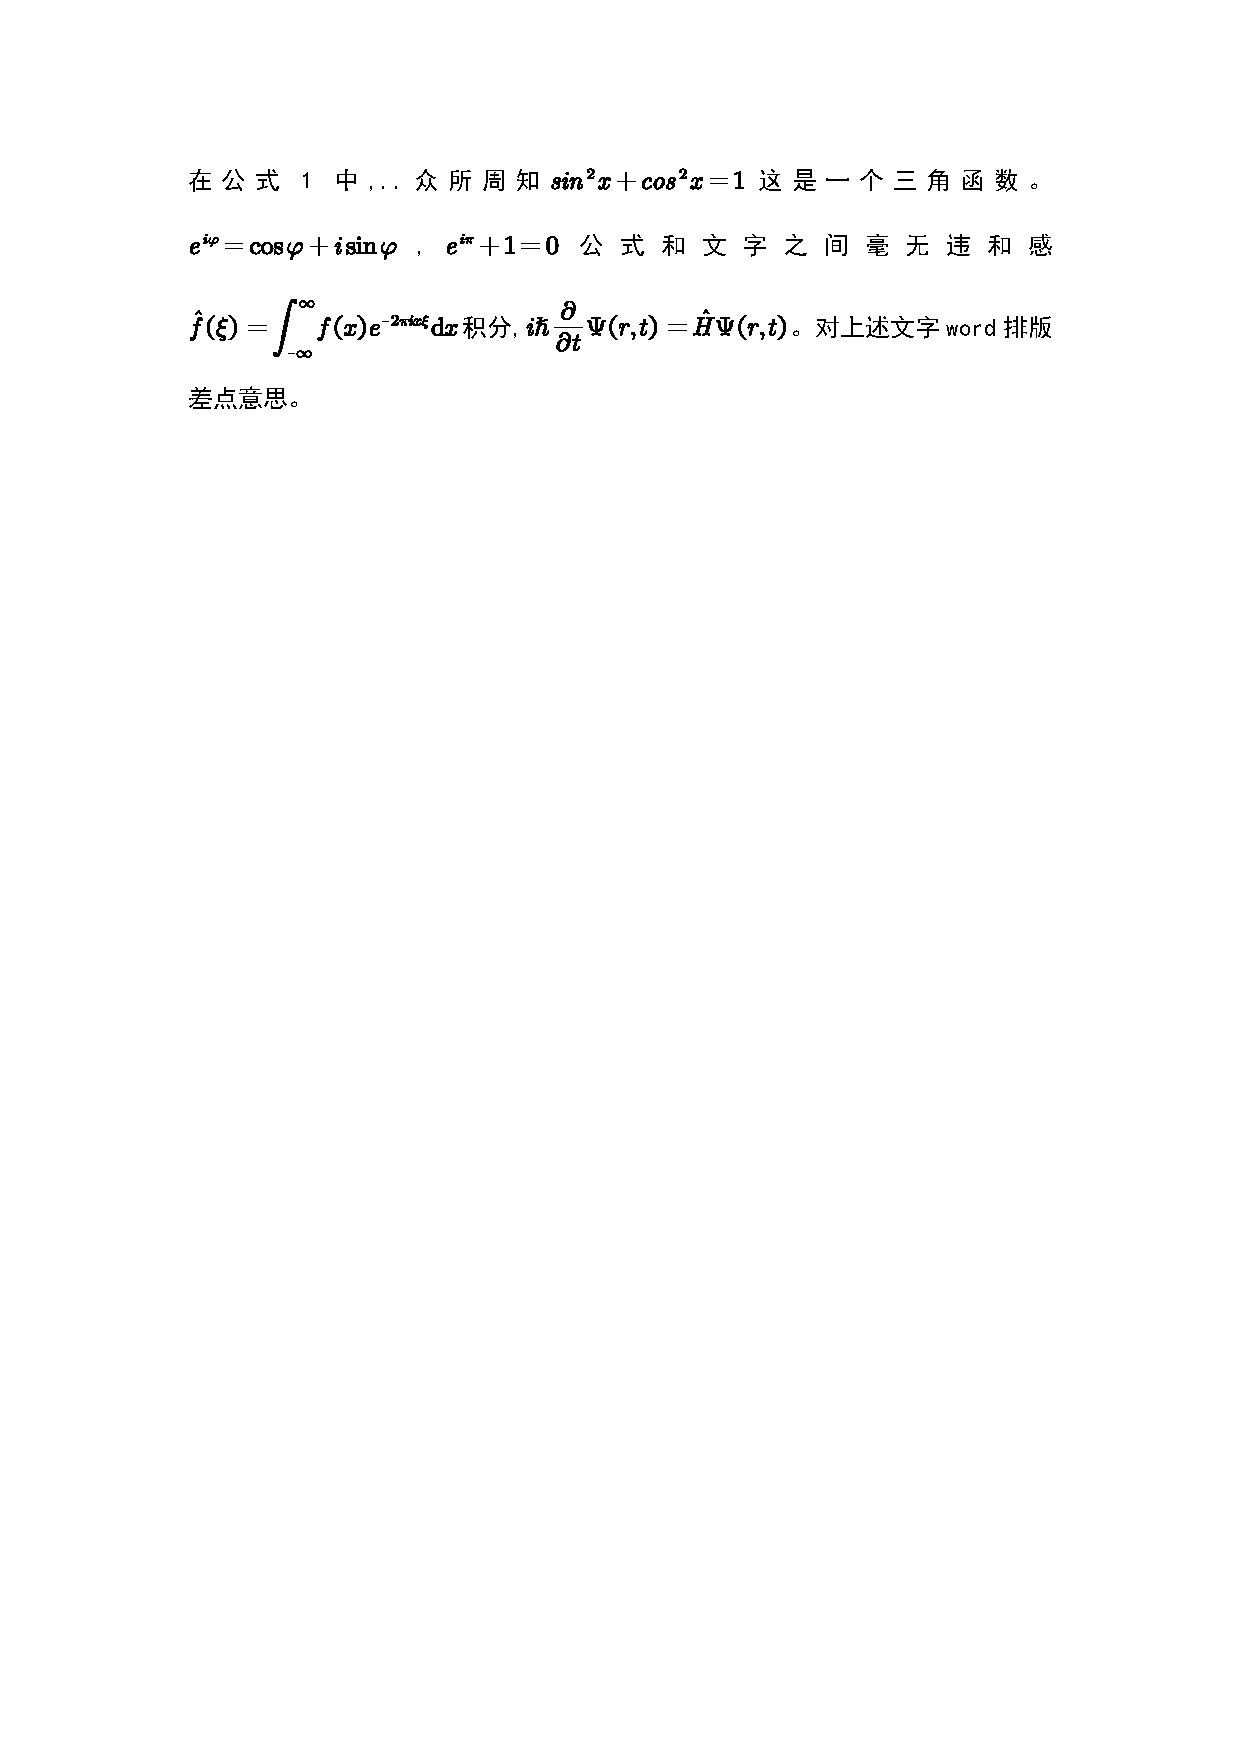
\includegraphics[width=8cm]{images/排版1.pdf}
			%\caption{}
			\label{fig:Figure3}
		\end{figure}
		
		\vspace{0cm} 
		\begin{figure}[h]
			\centering
			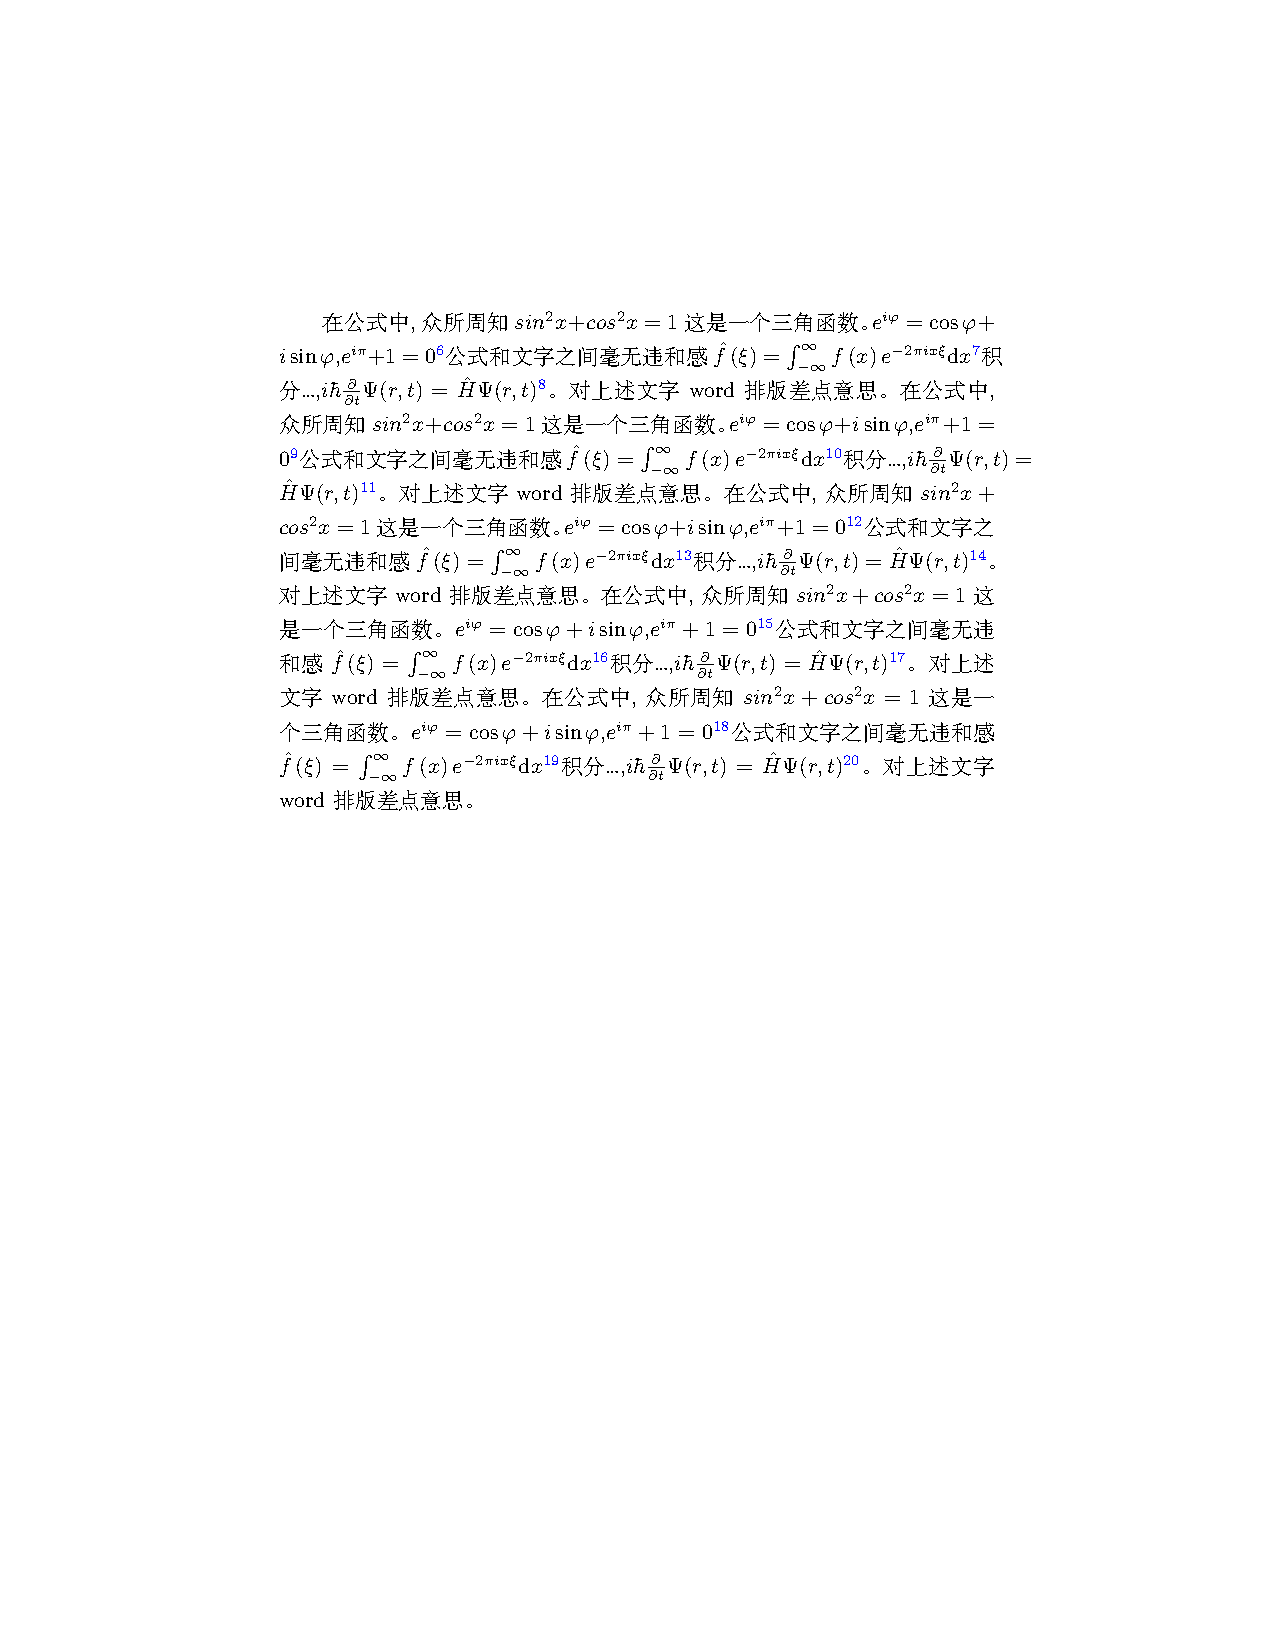
\includegraphics[width=10cm]{images/排版2.pdf}
			%\caption{}
			\label{fig:Figure4}
		\end{figure}
	
\end{frame}		

% --------- SECTION 3 ------- %
\section{学习MS}

\begin{frame}{MS}
	\begin{itemize}
		\item Functional:GGA-PBE~~LDA
		\begin{itemize}
			\item Geometry Optimization
			\item Energy
			\item Elastic
		\end{itemize}
	\end{itemize}
\end{frame}

\section{计划}
	\begin{frame}{计划}
		\begin{columns}
			\begin{column}{0.6\textwidth}
				\textbf{寒假计划}
					\begin{itemize}
						\item 学习\LaTeX
						\item 学习Python
						\item 学习英语
						\item 吃好玩好睡好\dots 
					\end{itemize}
			\end{column}
			
			\begin{column}{0.4\textwidth}
				\textbf{下学期计划}
					\begin{itemize}
						\item 完成课程学习不挂科
						\item 学习英语
						\item 学习MS
						\item “最好做点实验”...
					\end{itemize}
			\end{column}
		\end{columns}
\hyperlink{start}{\beamerreturnbutton{Back to start}}
	\end{frame}
\begin{frame}
	\begin{center}
		{\Huge\calligra Thank you!}
	\end{center}		
\end{frame}
		

\end{document}
